% Options for packages loaded elsewhere
\PassOptionsToPackage{unicode}{hyperref}
\PassOptionsToPackage{hyphens}{url}
%
\documentclass[
]{book}
\usepackage{amsmath,amssymb}
\usepackage{iftex}
\ifPDFTeX
  \usepackage[T1]{fontenc}
  \usepackage[utf8]{inputenc}
  \usepackage{textcomp} % provide euro and other symbols
\else % if luatex or xetex
  \usepackage{unicode-math} % this also loads fontspec
  \defaultfontfeatures{Scale=MatchLowercase}
  \defaultfontfeatures[\rmfamily]{Ligatures=TeX,Scale=1}
\fi
\usepackage{lmodern}
\ifPDFTeX\else
  % xetex/luatex font selection
\fi
% Use upquote if available, for straight quotes in verbatim environments
\IfFileExists{upquote.sty}{\usepackage{upquote}}{}
\IfFileExists{microtype.sty}{% use microtype if available
  \usepackage[]{microtype}
  \UseMicrotypeSet[protrusion]{basicmath} % disable protrusion for tt fonts
}{}
\makeatletter
\@ifundefined{KOMAClassName}{% if non-KOMA class
  \IfFileExists{parskip.sty}{%
    \usepackage{parskip}
  }{% else
    \setlength{\parindent}{0pt}
    \setlength{\parskip}{6pt plus 2pt minus 1pt}}
}{% if KOMA class
  \KOMAoptions{parskip=half}}
\makeatother
\usepackage{xcolor}
\usepackage{color}
\usepackage{fancyvrb}
\newcommand{\VerbBar}{|}
\newcommand{\VERB}{\Verb[commandchars=\\\{\}]}
\DefineVerbatimEnvironment{Highlighting}{Verbatim}{commandchars=\\\{\}}
% Add ',fontsize=\small' for more characters per line
\usepackage{framed}
\definecolor{shadecolor}{RGB}{248,248,248}
\newenvironment{Shaded}{\begin{snugshade}}{\end{snugshade}}
\newcommand{\AlertTok}[1]{\textcolor[rgb]{0.94,0.16,0.16}{#1}}
\newcommand{\AnnotationTok}[1]{\textcolor[rgb]{0.56,0.35,0.01}{\textbf{\textit{#1}}}}
\newcommand{\AttributeTok}[1]{\textcolor[rgb]{0.13,0.29,0.53}{#1}}
\newcommand{\BaseNTok}[1]{\textcolor[rgb]{0.00,0.00,0.81}{#1}}
\newcommand{\BuiltInTok}[1]{#1}
\newcommand{\CharTok}[1]{\textcolor[rgb]{0.31,0.60,0.02}{#1}}
\newcommand{\CommentTok}[1]{\textcolor[rgb]{0.56,0.35,0.01}{\textit{#1}}}
\newcommand{\CommentVarTok}[1]{\textcolor[rgb]{0.56,0.35,0.01}{\textbf{\textit{#1}}}}
\newcommand{\ConstantTok}[1]{\textcolor[rgb]{0.56,0.35,0.01}{#1}}
\newcommand{\ControlFlowTok}[1]{\textcolor[rgb]{0.13,0.29,0.53}{\textbf{#1}}}
\newcommand{\DataTypeTok}[1]{\textcolor[rgb]{0.13,0.29,0.53}{#1}}
\newcommand{\DecValTok}[1]{\textcolor[rgb]{0.00,0.00,0.81}{#1}}
\newcommand{\DocumentationTok}[1]{\textcolor[rgb]{0.56,0.35,0.01}{\textbf{\textit{#1}}}}
\newcommand{\ErrorTok}[1]{\textcolor[rgb]{0.64,0.00,0.00}{\textbf{#1}}}
\newcommand{\ExtensionTok}[1]{#1}
\newcommand{\FloatTok}[1]{\textcolor[rgb]{0.00,0.00,0.81}{#1}}
\newcommand{\FunctionTok}[1]{\textcolor[rgb]{0.13,0.29,0.53}{\textbf{#1}}}
\newcommand{\ImportTok}[1]{#1}
\newcommand{\InformationTok}[1]{\textcolor[rgb]{0.56,0.35,0.01}{\textbf{\textit{#1}}}}
\newcommand{\KeywordTok}[1]{\textcolor[rgb]{0.13,0.29,0.53}{\textbf{#1}}}
\newcommand{\NormalTok}[1]{#1}
\newcommand{\OperatorTok}[1]{\textcolor[rgb]{0.81,0.36,0.00}{\textbf{#1}}}
\newcommand{\OtherTok}[1]{\textcolor[rgb]{0.56,0.35,0.01}{#1}}
\newcommand{\PreprocessorTok}[1]{\textcolor[rgb]{0.56,0.35,0.01}{\textit{#1}}}
\newcommand{\RegionMarkerTok}[1]{#1}
\newcommand{\SpecialCharTok}[1]{\textcolor[rgb]{0.81,0.36,0.00}{\textbf{#1}}}
\newcommand{\SpecialStringTok}[1]{\textcolor[rgb]{0.31,0.60,0.02}{#1}}
\newcommand{\StringTok}[1]{\textcolor[rgb]{0.31,0.60,0.02}{#1}}
\newcommand{\VariableTok}[1]{\textcolor[rgb]{0.00,0.00,0.00}{#1}}
\newcommand{\VerbatimStringTok}[1]{\textcolor[rgb]{0.31,0.60,0.02}{#1}}
\newcommand{\WarningTok}[1]{\textcolor[rgb]{0.56,0.35,0.01}{\textbf{\textit{#1}}}}
\usepackage{longtable,booktabs,array}
\usepackage{calc} % for calculating minipage widths
% Correct order of tables after \paragraph or \subparagraph
\usepackage{etoolbox}
\makeatletter
\patchcmd\longtable{\par}{\if@noskipsec\mbox{}\fi\par}{}{}
\makeatother
% Allow footnotes in longtable head/foot
\IfFileExists{footnotehyper.sty}{\usepackage{footnotehyper}}{\usepackage{footnote}}
\makesavenoteenv{longtable}
\usepackage{graphicx}
\makeatletter
\def\maxwidth{\ifdim\Gin@nat@width>\linewidth\linewidth\else\Gin@nat@width\fi}
\def\maxheight{\ifdim\Gin@nat@height>\textheight\textheight\else\Gin@nat@height\fi}
\makeatother
% Scale images if necessary, so that they will not overflow the page
% margins by default, and it is still possible to overwrite the defaults
% using explicit options in \includegraphics[width, height, ...]{}
\setkeys{Gin}{width=\maxwidth,height=\maxheight,keepaspectratio}
% Set default figure placement to htbp
\makeatletter
\def\fps@figure{htbp}
\makeatother
\setlength{\emergencystretch}{3em} % prevent overfull lines
\providecommand{\tightlist}{%
  \setlength{\itemsep}{0pt}\setlength{\parskip}{0pt}}
\setcounter{secnumdepth}{5}
\usepackage{booktabs}
\ifLuaTeX
  \usepackage{selnolig}  % disable illegal ligatures
\fi
\usepackage[]{natbib}
\bibliographystyle{apalike}
\IfFileExists{bookmark.sty}{\usepackage{bookmark}}{\usepackage{hyperref}}
\IfFileExists{xurl.sty}{\usepackage{xurl}}{} % add URL line breaks if available
\urlstyle{same}
\hypersetup{
  pdftitle={pstratreg: An R package},
  pdfauthor={Ian Lundberg and Soonhong Cho},
  hidelinks,
  pdfcreator={LaTeX via pandoc}}

\title{pstratreg: An R package}
\author{Ian Lundberg and Soonhong Cho}
\date{2023-10-15}

\begin{document}
\maketitle

{
\setcounter{tocdepth}{1}
\tableofcontents
}
\hypertarget{welcome}{%
\chapter*{Welcome!}\label{welcome}}
\addcontentsline{toc}{chapter}{Welcome!}

\begin{quote}
\textbf{WARNING.} This website documents an R package that is in development. Expect changes. We encourage you to try the package and email us with suggestions.\footnote{Ian Lundberg (\href{mailto:ilundberg@cornell.edu}{\nolinkurl{ilundberg@cornell.edu}}) and Soonhong Cho (\href{mailto:soonhongcho@g.ucla.edu}{\nolinkurl{soonhongcho@g.ucla.edu}})}
\end{quote}

This website documents the \textbf{pstratreg} package for R. The package helps study causal effects when some treatment values cause outcomes to be non-existent for some units.

Possible applications include

\begin{itemize}
\tightlist
\item
  a labor market intervention where the outcome is hourly wage, but some people are unemployed
\item
  a medical intervention where the outcome is a health metric, but some people die before it is measured
\item
  a sociological study where the outcome involves one's spouse, but some people divorce or never marry and thus have no spouse
\end{itemize}

This package provides regression-based methods for principal stratification that rely on parametric models and are useful in settings where one hopes to adjust for many confounders.

\hypertarget{getting-started}{%
\section*{Getting started}\label{getting-started}}
\addcontentsline{toc}{section}{Getting started}

To get started, first install \href{https://rstudio-education.github.io/hopr/starting.html}{R and RStudio}. Then install the package.

\begin{Shaded}
\begin{Highlighting}[]
\NormalTok{devtools}\SpecialCharTok{::}\FunctionTok{install\_github}\NormalTok{(}\StringTok{"ilundberg/pstratreg"}\NormalTok{)}
\end{Highlighting}
\end{Shaded}

Now head on to the next page to see the types of questions this package can help answer.

This project is joint work between Ian Lundberg (Cornell, \href{mailto:ilundberg@cornell.edu}{\nolinkurl{ilundberg@cornell.edu}}) and Soonhong Cho (UCLA, \href{mailto:soonhongcho@g.ucla.edu}{\nolinkurl{soonhongcho@g.ucla.edu}}).

\hypertarget{the-goal}{%
\chapter{The goal}\label{the-goal}}

Average causal effects are undefined when some outcomes do not exist. For example, consider the two people below who were eligible for a job training intervention.

\begin{longtable}[]{@{}
  >{\centering\arraybackslash}p{(\columnwidth - 6\tabcolsep) * \real{0.2500}}
  >{\centering\arraybackslash}p{(\columnwidth - 6\tabcolsep) * \real{0.2500}}
  >{\centering\arraybackslash}p{(\columnwidth - 6\tabcolsep) * \real{0.2500}}
  >{\centering\arraybackslash}p{(\columnwidth - 6\tabcolsep) * \real{0.2500}}@{}}
\toprule\noalign{}
\begin{minipage}[b]{\linewidth}\centering
Person
\end{minipage} & \begin{minipage}[b]{\linewidth}\centering
Wage with job training
\end{minipage} & \begin{minipage}[b]{\linewidth}\centering
Wage without job training
\end{minipage} & \begin{minipage}[b]{\linewidth}\centering
Causal effect
\end{minipage} \\
\midrule\noalign{}
\endhead
\bottomrule\noalign{}
\endlastfoot
Javier & \$30 & \$20 & \$30-\$20=\$10 \\
William & \$26 & ?? & \$30-??=?? \\
\textbf{Average} & \textbf{\$28} & \textbf{??} & \textbf{??} \\
\end{longtable}

A social scientist might study the average causal effect of the intervention on future hourly wages. But without job training, William would not be employed at all. His wage ?? does not exist. As a result, the average causal effect does not exist. Principal stratification is a method to estimate average causal effects in the subpopulation that excludes people like William, for whom the effect is undefined.

\begin{quote}
\textbf{Where to read more.} For original ideas, see \href{https://doi.org/10.1111/j.0006-341X.2002.00021.x}{Frangakis \& Rubin (2002)} and \href{https://doi.org/10.3102/10769986028004353}{Zhang \& Rubin (2003)}. For a recent introduction, see \href{https://doi.org/10.1080/19345747.2017.1379576}{Miratrix et al.~(2018)}.
\end{quote}

This page is a tutorial on the ideas behind principal stratification. The next page discusses the regression setting that is the focus of this package. Subsequent pages show package functionality.

\hypertarget{defining-principal-strata}{%
\section{Defining principal strata}\label{defining-principal-strata}}

Let \(M_i\) be a binary mediator (e.g., employment) that determines whether an outcome exists for unti \(i\). Let \(Y_i\) be the outcome, where \(Y\) is undefined when \(M = 0\). Let \(\{M_i^1,M_i^0\}\) and \(\{Y_i^1,Y_i^0\}\) be the potential values that the mediator and outcome would take for unit \(i\) under job training and under no job training. The table above gave values for \(\{Y_i^1,Y_i^0\}\).

Define four \textbf{principal strata} of units by the effect that the intervention has on the mediator value

\begin{longtable}[]{@{}
  >{\centering\arraybackslash}p{(\columnwidth - 4\tabcolsep) * \real{0.3333}}
  >{\centering\arraybackslash}p{(\columnwidth - 4\tabcolsep) * \real{0.3333}}
  >{\centering\arraybackslash}p{(\columnwidth - 4\tabcolsep) * \real{0.3333}}@{}}
\toprule\noalign{}
\begin{minipage}[b]{\linewidth}\centering
Stratum
\end{minipage} & \begin{minipage}[b]{\linewidth}\centering
Math
\end{minipage} & \begin{minipage}[b]{\linewidth}\centering
English
\end{minipage} \\
\midrule\noalign{}
\endhead
\bottomrule\noalign{}
\endlastfoot
\(S_i = \text{Always}\) & \(M_i^1 = M_i^0 = 1\) & Always employed, regardless of the intervention \\
\(S_i = \text{Induced}\) & \(M_i^1 > M_i^0\) & Induced into employment by the intervention \\
\(S_i = \text{Blocked}\) & \(M_i^1 < M_i^0\) & Blocked from employment by the intervention \\
\(S_i = \text{Never}\) & \(M_i^1 = M_i^0 = 0\) & Never employed, regardless of the intervention \\
\end{longtable}

In our example, Javier is a member of the always stratum and William is a member of the induced stratum.

\hypertarget{target-population-the-always-stratum}{%
\section{Target population: The always stratum}\label{target-population-the-always-stratum}}

The average causal effect \(E(Y^1 - Y^0)\) is only defined in the ``Always'' stratum.

\begin{itemize}
\tightlist
\item
  in the induced stratum, \(Y^0\) is undefined, so the effect is \(Y^1 - ??\)
\item
  in the blocked stratum, \(Y^1\) is undefined, so the effect is \(?? - Y^0\)
\item
  in the never stratum, both are undefined, so the effect is \(?? - ??\)
\end{itemize}

Our causal estimand is therefore the average causal effect in the always stratum.

\[E(Y^1 - Y^0 \mid S = \text{Always})\]

\hypertarget{fundamental-problem-strata-are-latent}{%
\section{Fundamental problem: Strata are latent}\label{fundamental-problem-strata-are-latent}}

Suppose William received job training. We would observe his \$26 wage. We would not know that he would not have been employed without job training. If William received job training, then in the observed data we would know that he was either in the always stratum or the induced stratum.

What can be observed is the treatment value \(D_i\) and the mediator value \(M_i\). Each combination of these values is a mixture of two principal strata.

\begin{longtable}[]{@{}ccc@{}}
\toprule\noalign{}
& \(D_i = 1\) & \(D_i = 0\) \\
\midrule\noalign{}
\endhead
\bottomrule\noalign{}
\endlastfoot
\(M_i = 1\) & Always and Induced & Always and Blocked \\
\(M_i = 0\) & Never and Blocked & Never and Induced \\
\end{longtable}

\hypertarget{solution-step-1-make-an-assumption}{%
\section{Solution step 1: Make an assumption}\label{solution-step-1-make-an-assumption}}

Assumptions can simplify the problem, and can be plausible in some settings. We focus on two versions of one assumption.

\begin{longtable}[]{@{}ccc@{}}
\toprule\noalign{}
Assumption & Math & English \\
\midrule\noalign{}
\endhead
\bottomrule\noalign{}
\endlastfoot
Positive monotonicity & \(M_i^1 \geq M_i^0\) & No one is blocked \\
Negative monotonicity & \(M_i^1\leq M_i^0\) & No one is induced \\
\end{longtable}

In our example, the positive monotonicity assumption may be credible: job training is unlikely to block anyone from employment. In other settings, the negative monotonicity assumption is credible. If the treatment were having a criminal record on one's resume, that treatment might block employment but would be unlikely to induce employment.

Under positive monotonicity, some latent strata become observable.

\begin{longtable}[]{@{}ccc@{}}
\toprule\noalign{}
& \(D_i = 1\) & \(D_i = 0\) \\
\midrule\noalign{}
\endhead
\bottomrule\noalign{}
\endlastfoot
\(M_i = 1\) & Always and Induced & Always \\
\(M_i = 0\) & Never & Never and Induced \\
\end{longtable}

For example, suppose that Javier was assigned to no job training, and we observed that he was employed. Under positive monotonicity, we would know that Javier was in the always stratum because he was employed without job training, and thus surely would have been employed with job training.

\hypertarget{solution-step-2-bound-the-average-effect-in-the-always-stratum}{%
\section{Solution step 2: Bound the average effect in the always stratum}\label{solution-step-2-bound-the-average-effect-in-the-always-stratum}}

Suppose we assume positive monotonicity, and we observe data where four people have been randomized to each treatment condition.

In the no-job-training condition, we observe the following four people

\begin{longtable}[]{@{}cccc@{}}
\toprule\noalign{}
Person & Treatment & Wage & Stratum \\
\midrule\noalign{}
\endhead
\bottomrule\noalign{}
\endlastfoot
Jamal & No job training & \$20 & Always \\
Sandra & No job training & \$16 & Always \\
Oscar & No job training & ?? & Never or Induced \\
Nancy & No job training & ?? & Never or Induced \\
\end{longtable}

The stratum column is sometimes known by assumption: Jamal and Sandra were employed despite no job training, so they surely would have been employed in a counterfactual world with job training (by positive monotonicity). Oscar and Nancy might or might not have been employed in a counterfactual world where they received job training.

Four people were randomized to the treatment: job training

\begin{longtable}[]{@{}cccc@{}}
\toprule\noalign{}
Person & Treatment & Wage & Stratum \\
\midrule\noalign{}
\endhead
\bottomrule\noalign{}
\endlastfoot
Nia & Job training & \$40 & Always or Induced \\
Steven & Job training & \$32 & Always or Induced \\
Maya & Job training & \$29 & Always or Induced \\
Hugo & Job training & \$25 & Always or Induced \\
\end{longtable}

The stratum column for the four treated people is always unknown, because under positive monotonicity they might or might not have been employed despite no job training.

By comparing the frequency of ?? in the tables, we can estimate that job training reduces employment by 50 percentage points. This tells us the size of the induced stratum.

\[\hat{P}(S = \text{Induced}) = 0.5\]

Because all those receiving job training were employed, our data also suggest that the never-employed stratum is empty.

\[\hat{P}(S = \text{Never}) = 0\]

Thus, in our example we estimate that 50\% of people are always employed and 50\% would be induced into employment if exposed to job training. Thus half of \{Nia, Steven, Maya, Hugo\} are always-employed.

But which half? This is impossible to know. We therefore \textbf{bound} the expected outcome under treatment.

\begin{itemize}
\tightlist
\item
  for an \emph{upper bound}, assume the highest-valued half of the treated units are the always-employed ones

  \begin{itemize}
  \tightlist
  \item
    Nia and Steven are always employed
  \item
    Maya and Hugo are induced
  \item
    \(\hat{E}_\text{Upper}(Y^1\mid S = \text{Always}) = \frac{32+40}{2} = \$36\)
  \end{itemize}
\item
  for a \emph{lower bound}, assume the lowest-valued half of the treated units are the always-employed ones

  \begin{itemize}
  \tightlist
  \item
    Nia and Steven are induced
  \item
    Maya and Hugo are always employed
  \item
    \(\hat{E}_\text{Lower}(Y^1\mid S = \text{Always}) = \frac{25+29}{2} = \$27\)
  \end{itemize}
\end{itemize}

Because under positive monotonicity all untreated individuals must be always-employed, we point estimate the outcome under control

\[\hat{E}(Y^0\mid S = \text{Always}) = \$18\]

The difference tells us that the average causal effect of job training on the wages of the always employed is between \$27 - \$18 = \$9 and \$36 - \$18 = \$18.

\hypertarget{why-regression}{%
\chapter{Why regression}\label{why-regression}}

The goal of this package is to support parametric model-based principal stratification. This page motivates that choice: why should we want a model?

Parametric regression models make principal stratification bounds applicable in social science settings with many covariates. One such setting is causal inference in observational settings. In that setting, we might want to statistically adjust for a covariate vector \(\vec{X}\).

\begin{itemize}
\tightlist
\item
  when \(\vec{X}\) can take only a few discrete values, one can carry out principal stratification as above within each stratum of \(\vec{X}\)
\item
  when \(\vec{X}\) can take many values, it is possible that each vector value \(\vec{X}_i\) is unique
\end{itemize}

In the latter case, we need model-based principal stratification.

\begin{enumerate}
\def\labelenumi{\arabic{enumi})}
\tightlist
\item
  Model the mediator

  \begin{itemize}
  \tightlist
  \item
    Fit a model for the mediator \(M\)
  \item
    Estimate the probability of each stratum for each unit
  \end{itemize}
\item
  Model the outcome

  \begin{itemize}
  \tightlist
  \item
    Fit a model for the outcome \(Y\mid A = 1, M = 1, \vec{X}\)

    \begin{itemize}
    \tightlist
    \item
      Example: Model the distribution of wages for employed job training recipients
    \end{itemize}
  \item
    Fit a model for the outcome \(Y\mid A = 0, M = 1, \vec{X}\)

    \begin{itemize}
    \tightlist
    \item
      Example: Model the distribution of wages for employed job training recipients
    \end{itemize}
  \item
    Bound by assuming that the proportion induced (from 1) is the upper or lower portion conditional on covariates
  \end{itemize}
\end{enumerate}

\hypertarget{upper-bound-left---right}{%
\subsection{Upper bound: Left - Right}\label{upper-bound-left---right}}

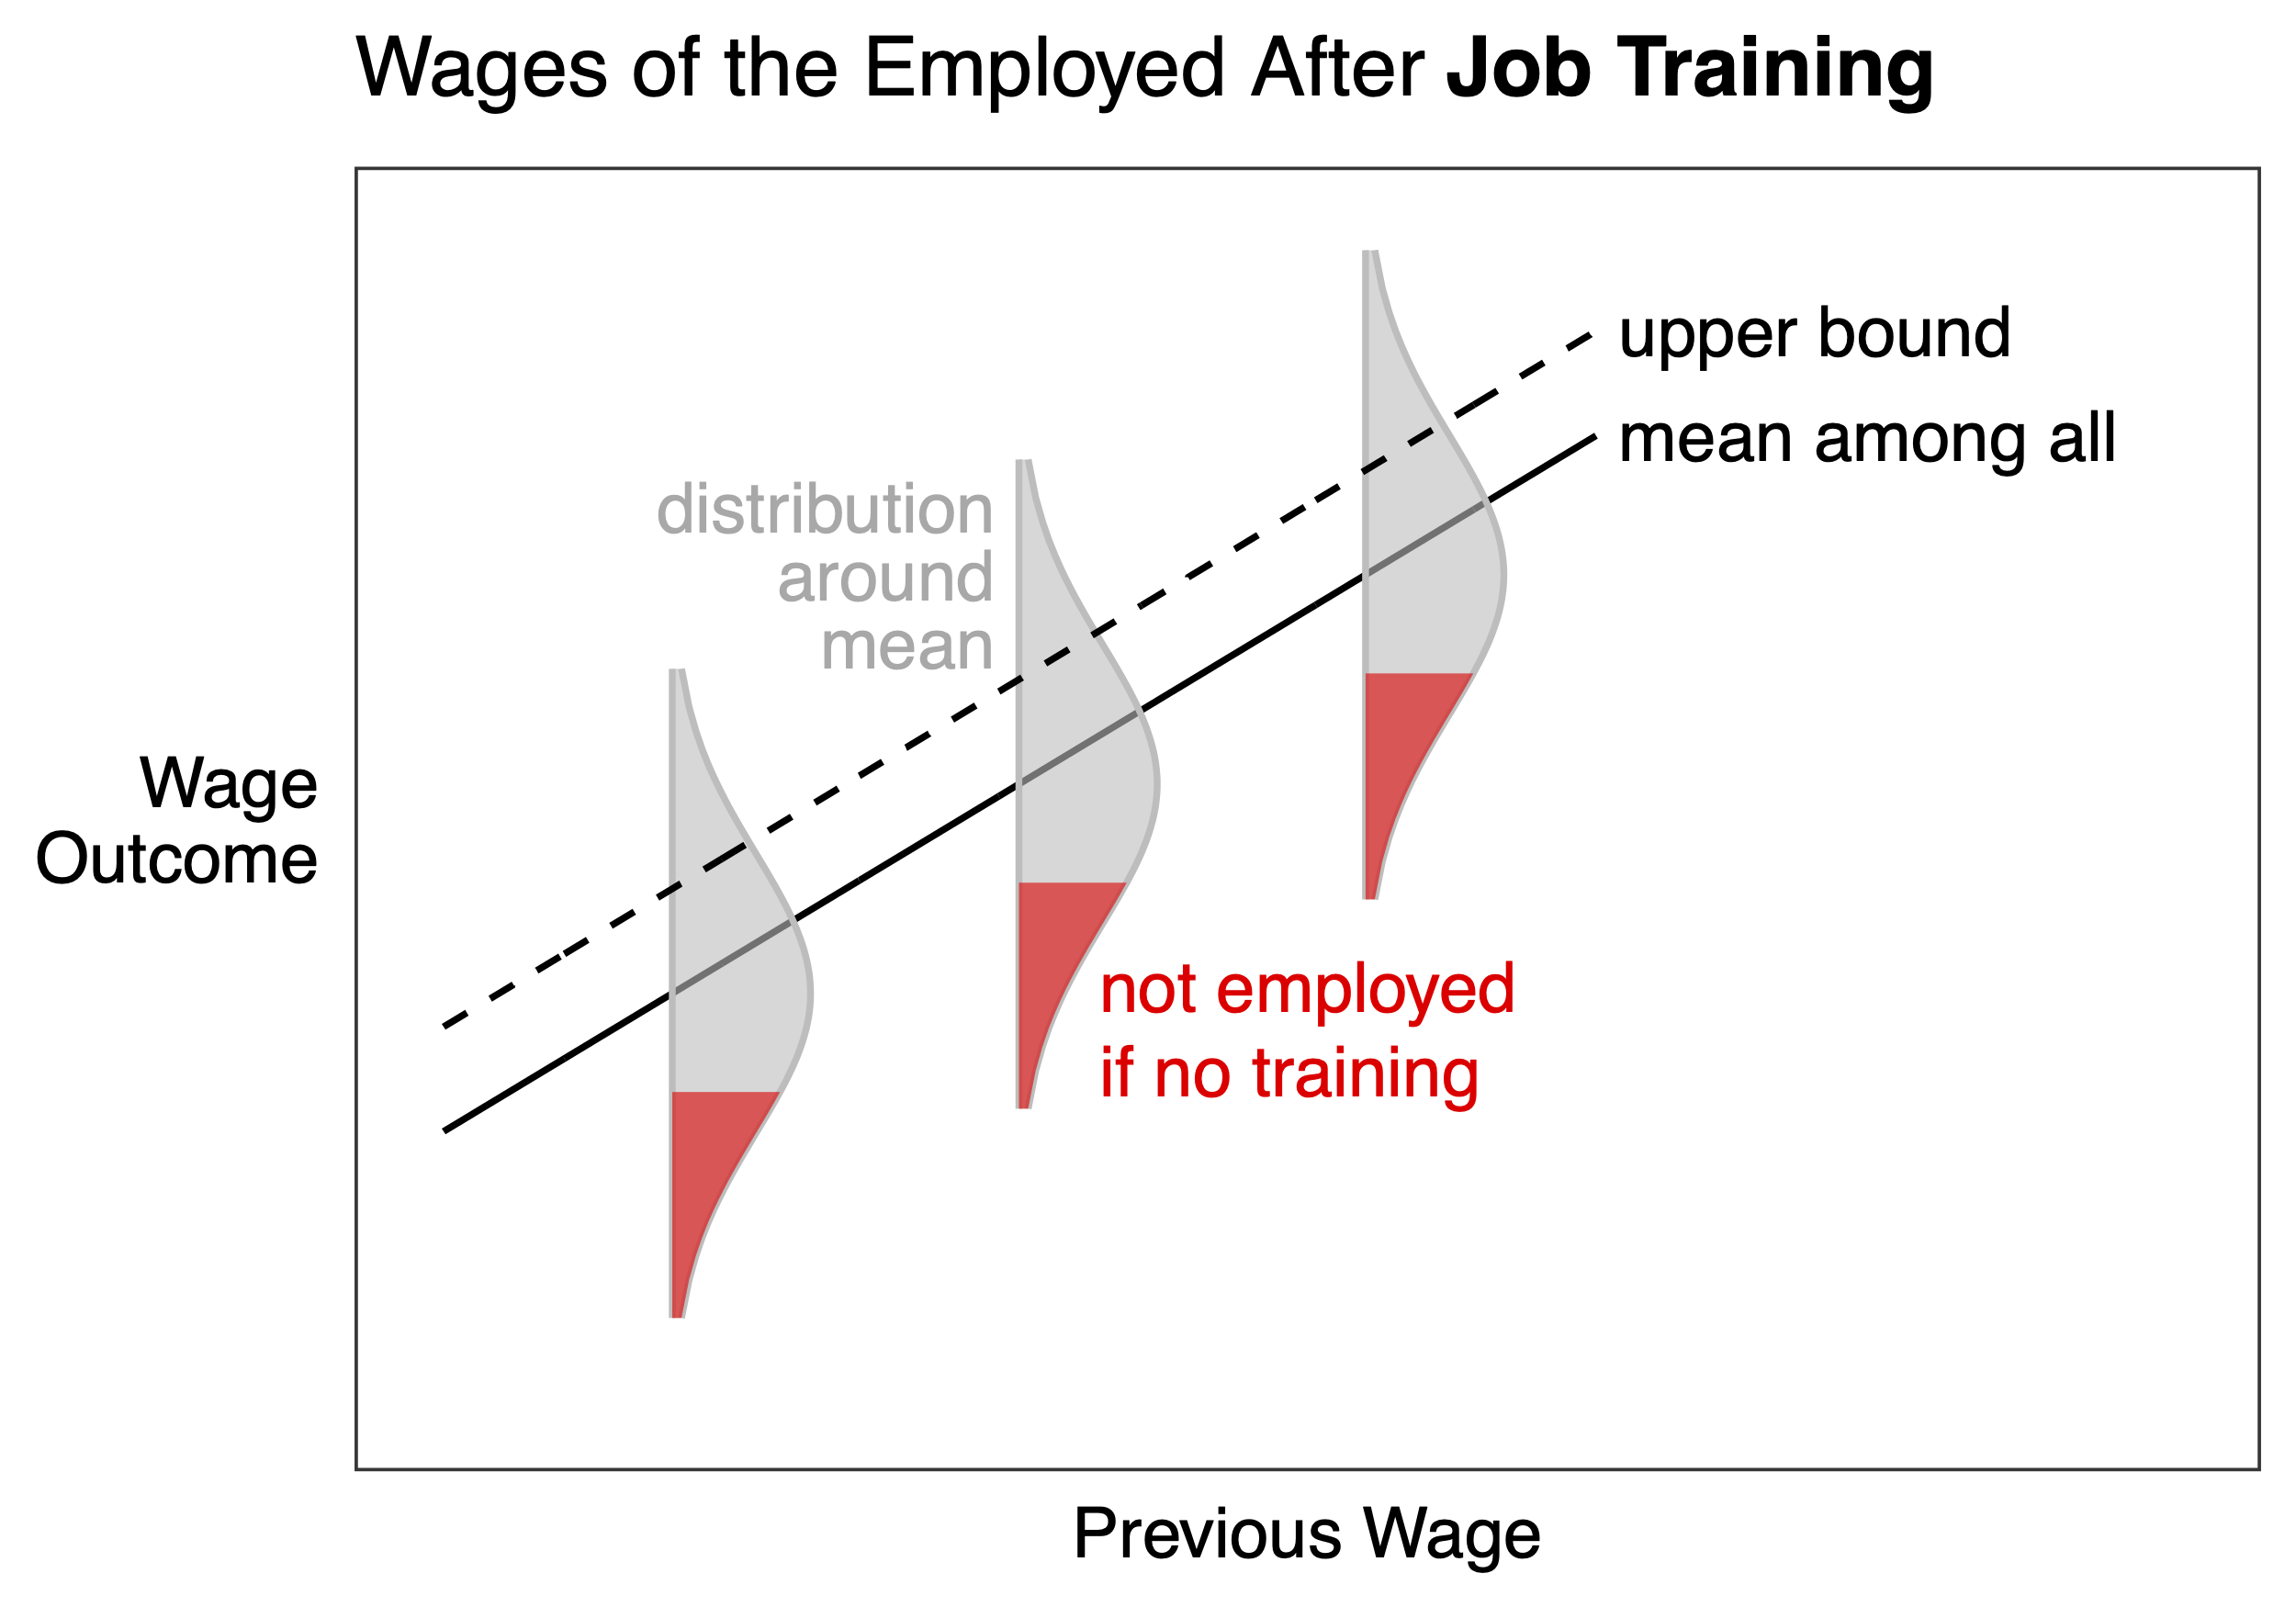
\includegraphics[width=0.4\textwidth,height=\textheight]{assets/teach_jobtrain_upper.png}
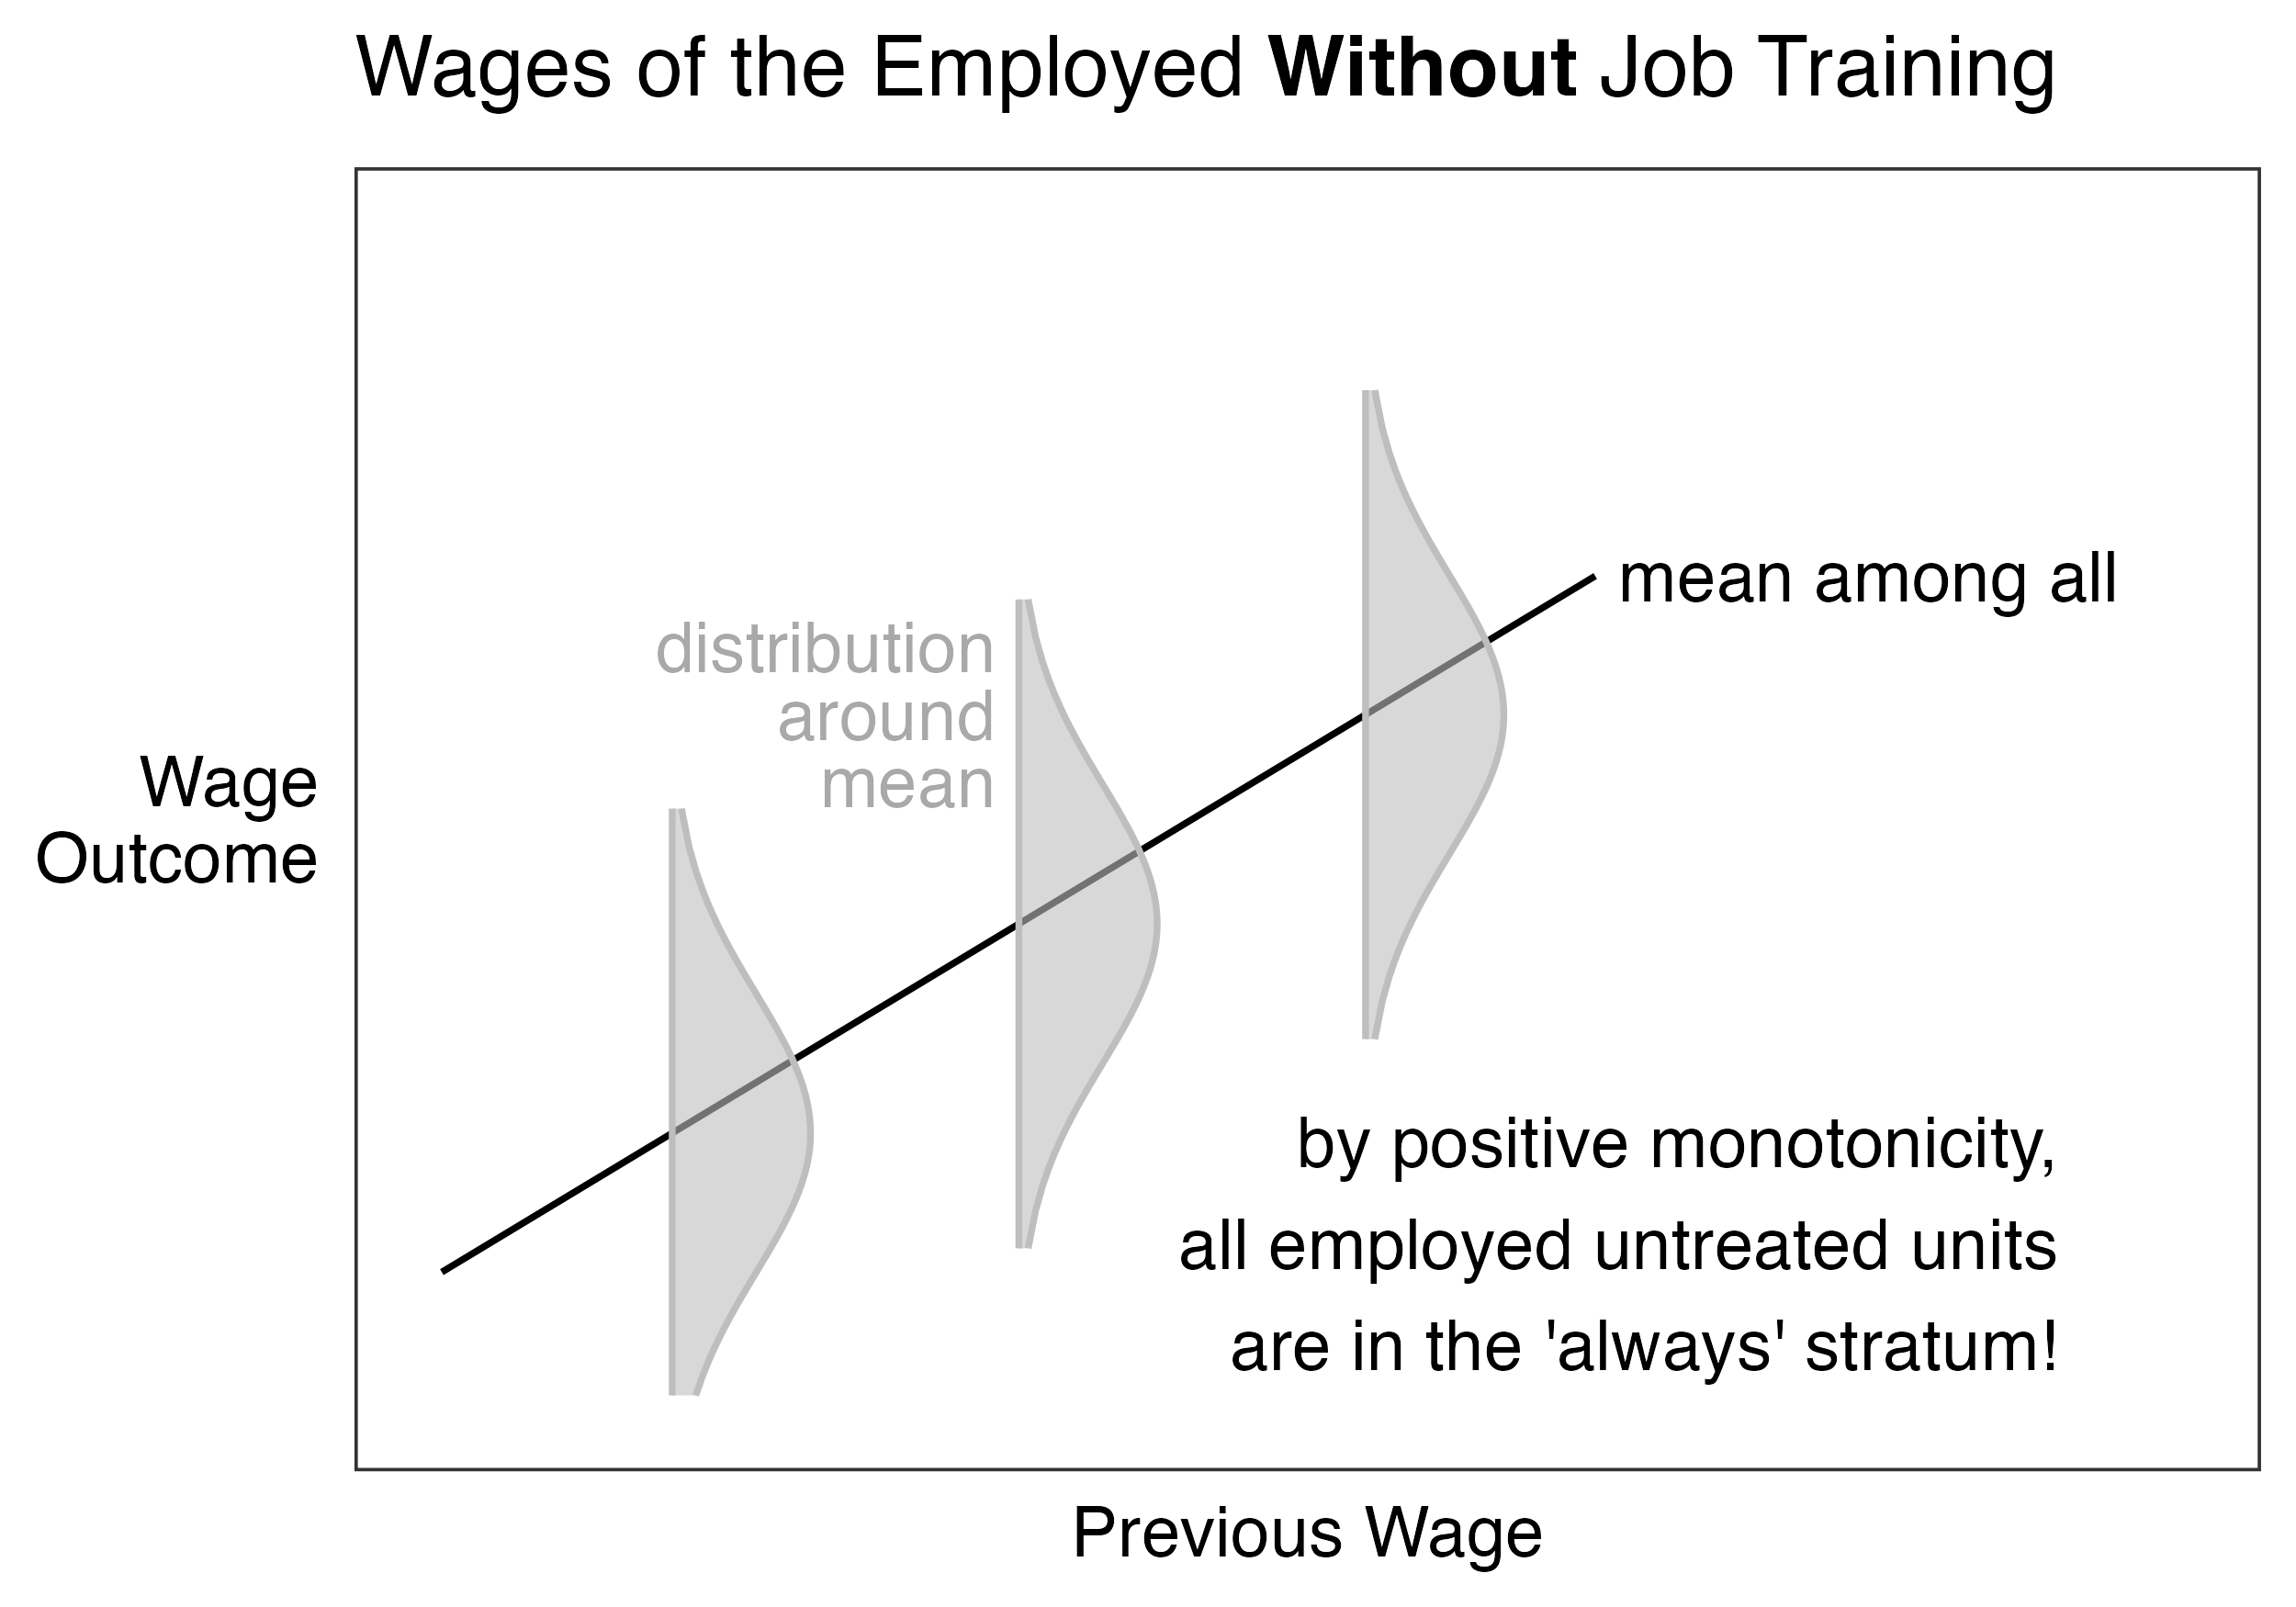
\includegraphics[width=0.4\textwidth,height=\textheight]{assets/teach_jobtrain_control.png}

\hypertarget{lower-bound-left---right}{%
\subsection{Lower bound: Left - Right}\label{lower-bound-left---right}}

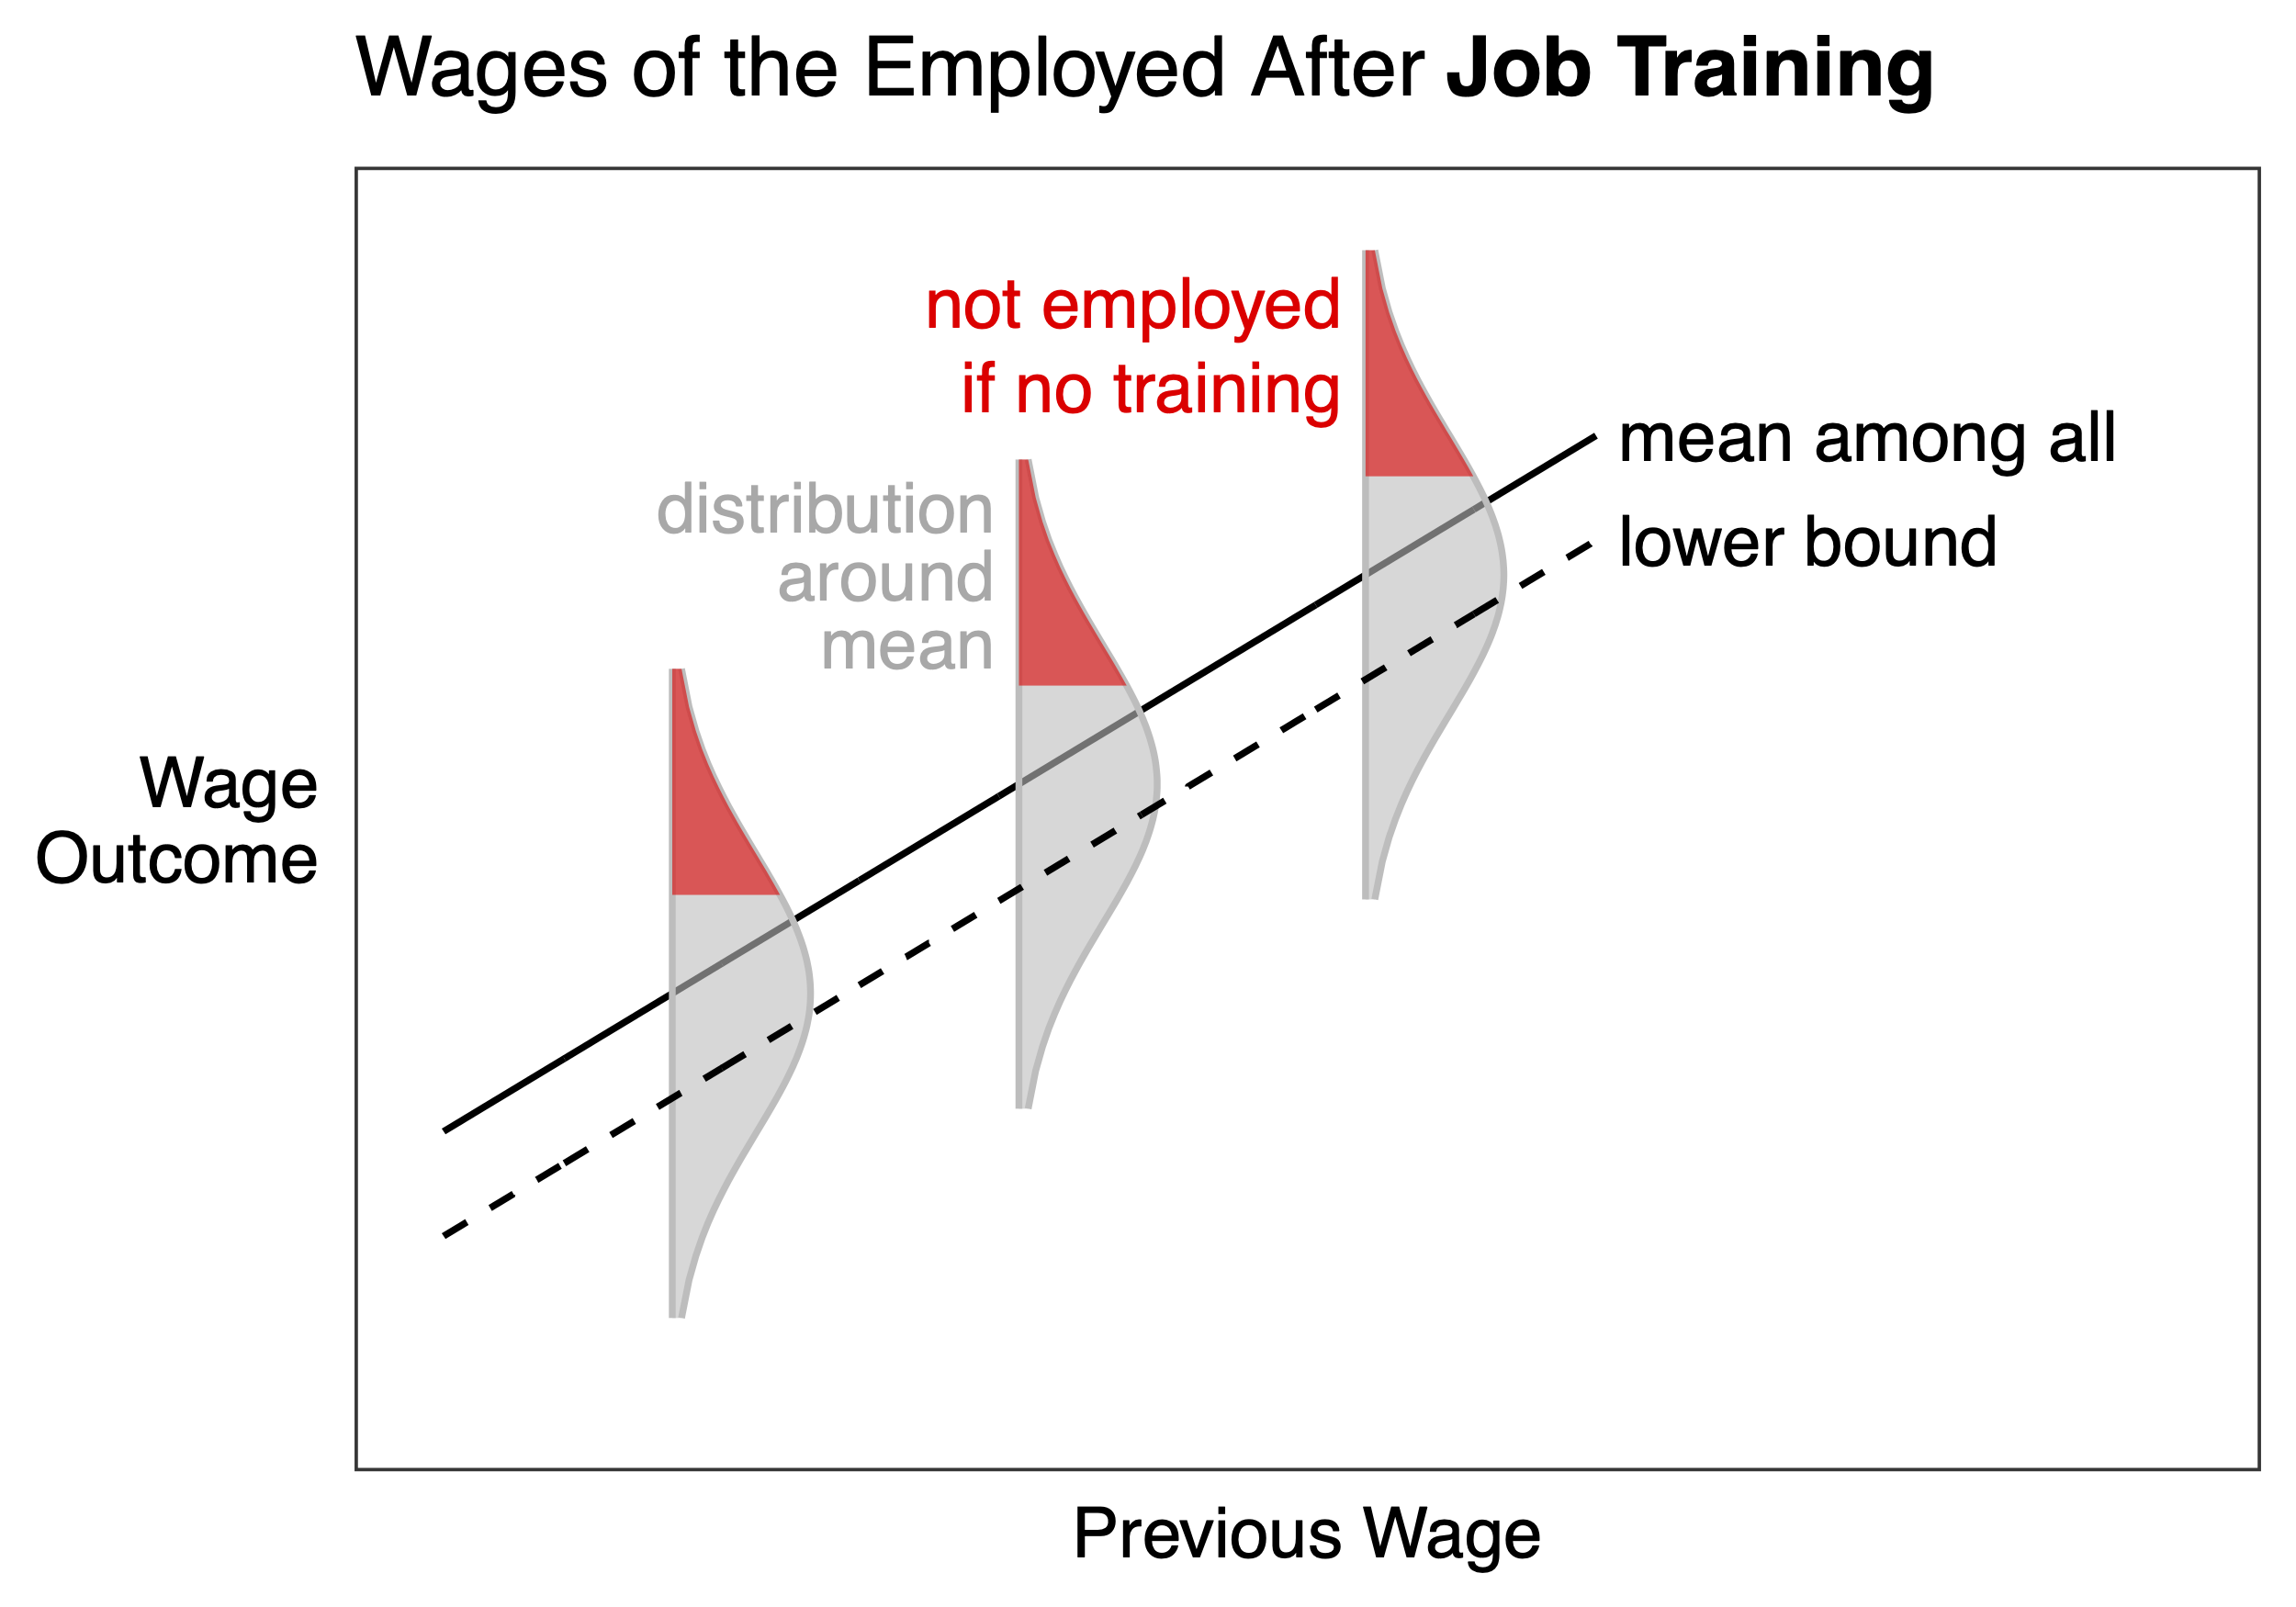
\includegraphics[width=0.4\textwidth,height=\textheight]{assets/teach_jobtrain_lower.png}
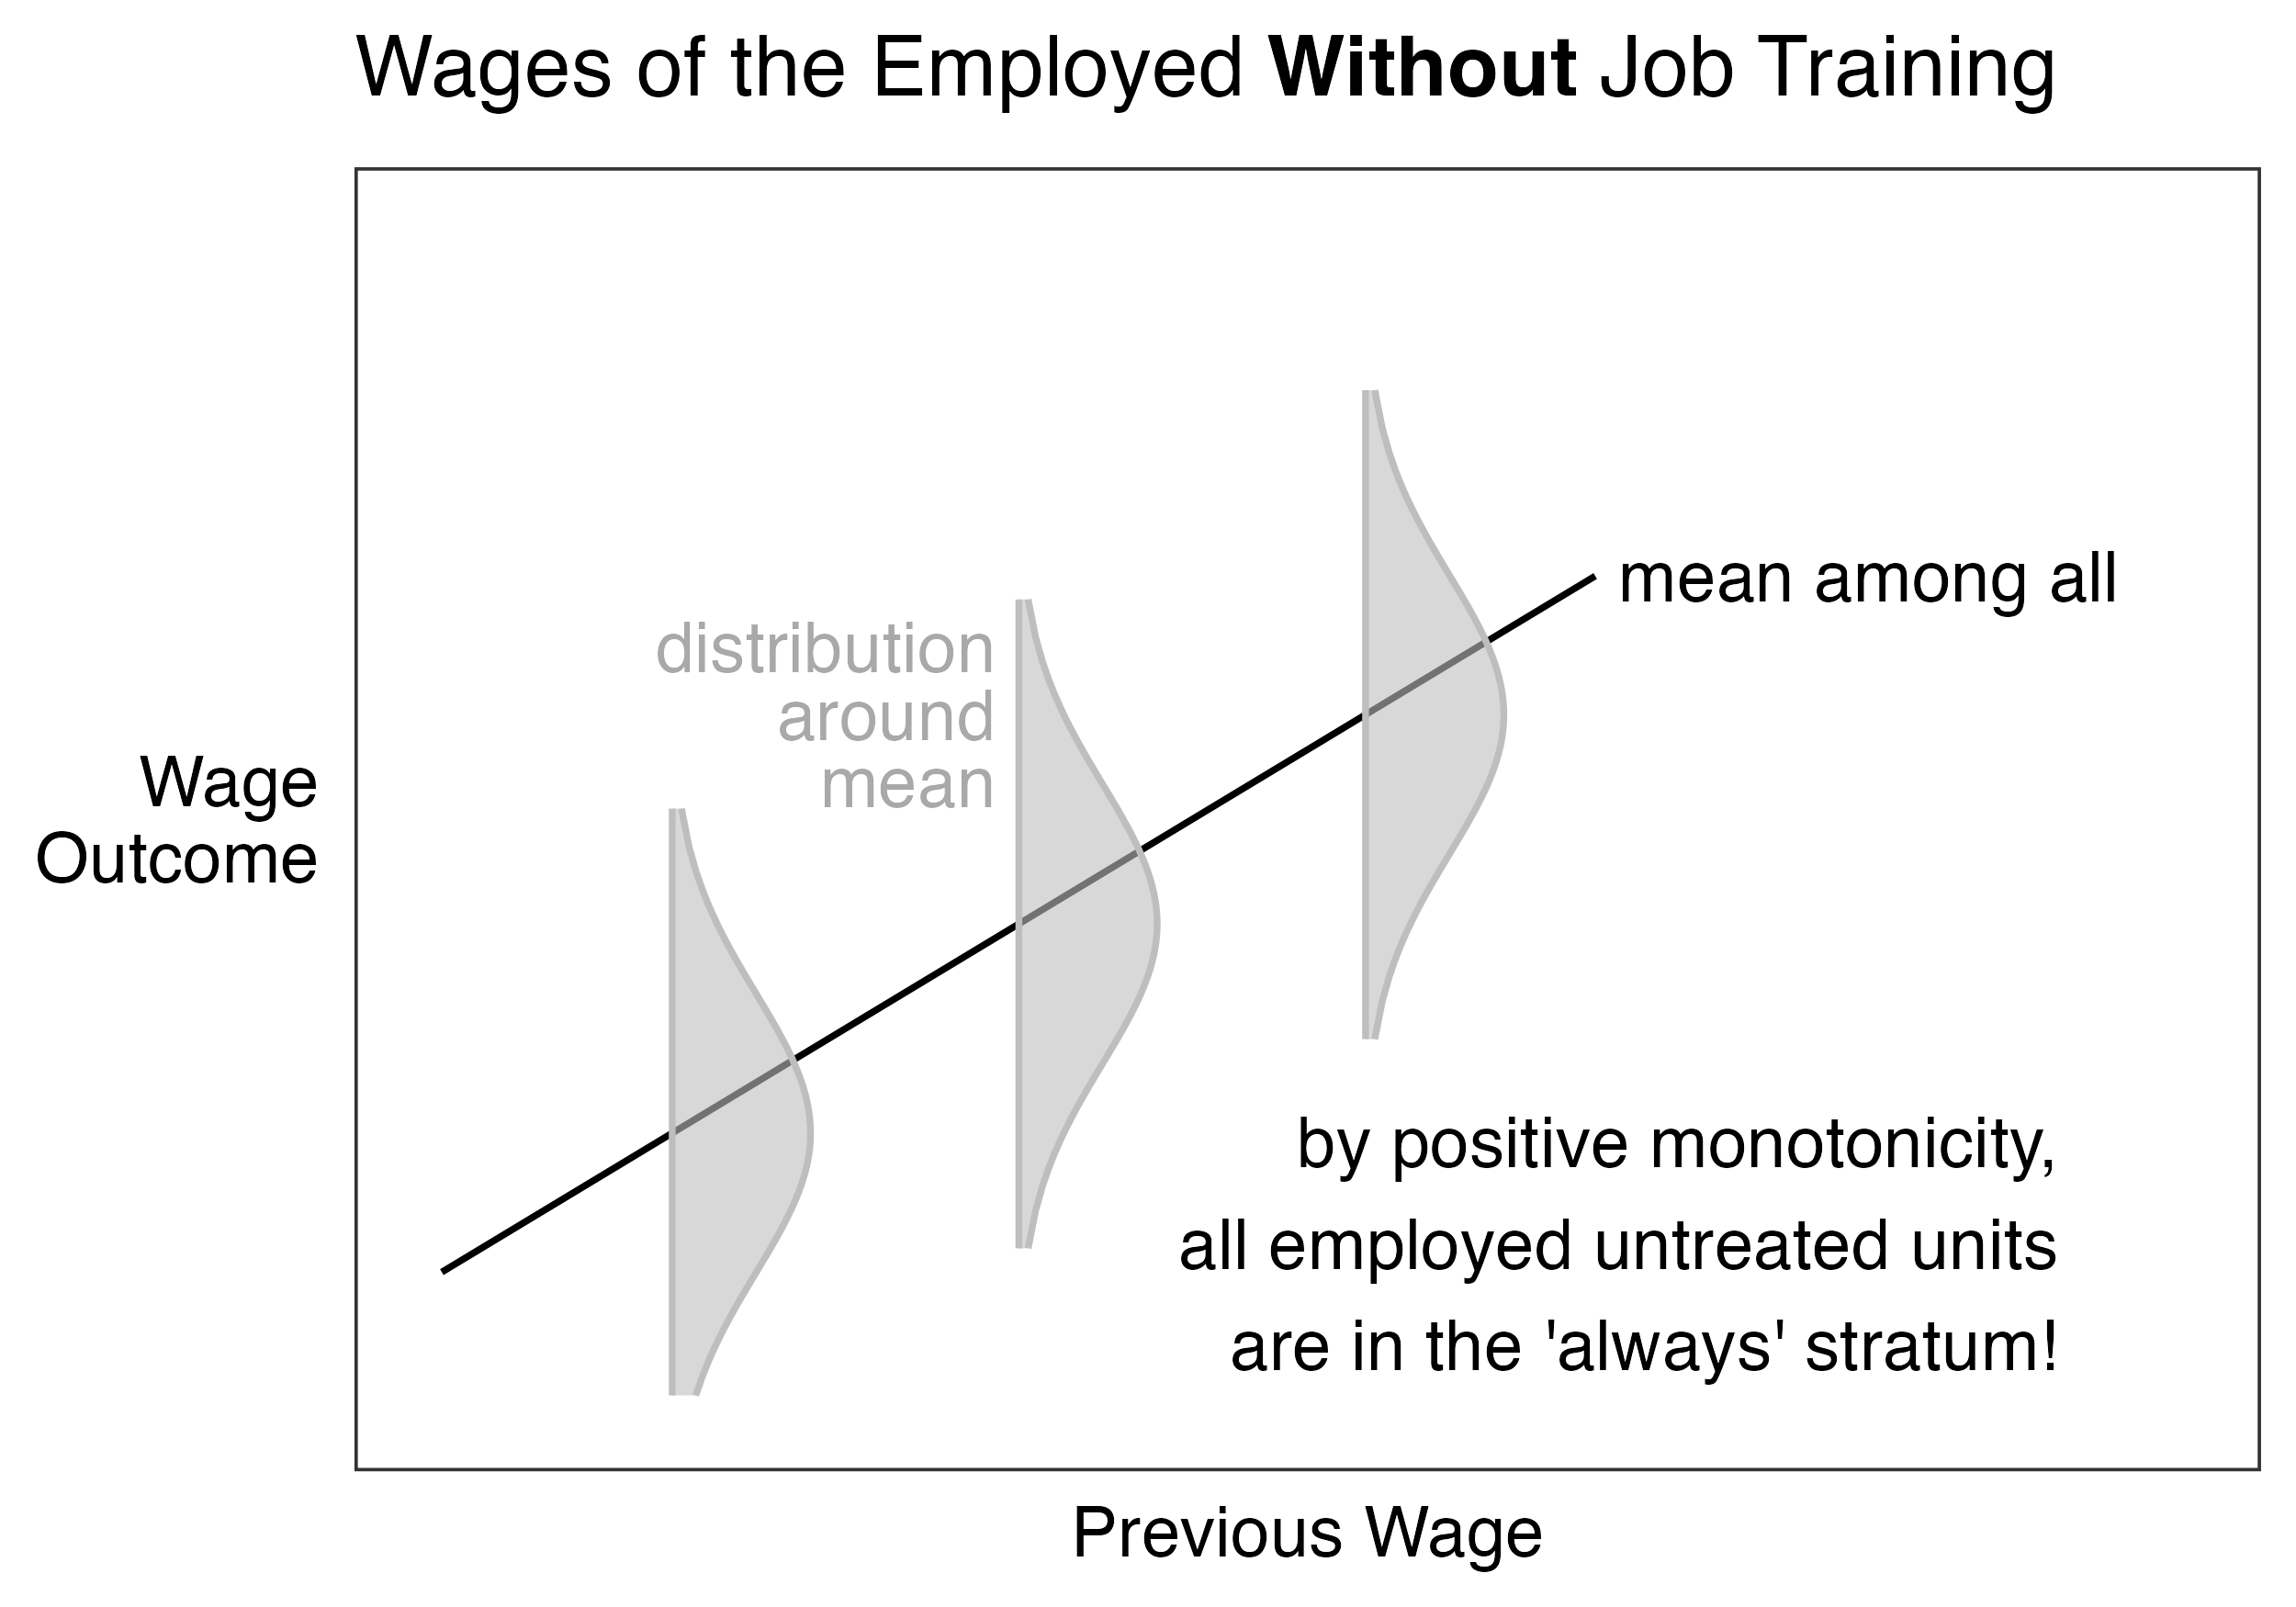
\includegraphics[width=0.4\textwidth,height=\textheight]{assets/teach_jobtrain_control.png}

\hypertarget{basic-functionality}{%
\chapter{Basic functionality}\label{basic-functionality}}

This page illustrates the basic functionality of the \texttt{pstratreg} function. This function conducts parametric principal stratification analysis to estimate average causal effect among the always-valid subgroup whose outcome would exist in either treatment condition.

\begin{quote}
Jargon? Start with the first page on \protect\hyperlink{the-goal}{the goal}!
\end{quote}

The package automates the process to

\begin{itemize}
\tightlist
\item
  estimate a mediator model
\item
  estimate an outcome model

  \begin{itemize}
  \tightlist
  \item
    allowing heteroskedasticity if needed
  \end{itemize}
\item
  calculate the conditional probability of being always-valid
\item
  implement monotonicity assumptions
\item
  bound estimates using the conditional outcome distribution and the proportion in the always-valid subgroup
\item
  return estimates, conditional on population subgroups if requested
\end{itemize}

\hypertarget{simulate-data}{%
\section{Simulate data}\label{simulate-data}}

We first simulate some data for illustration.

The data has four variables

\begin{itemize}
\tightlist
\item
  continuous confounder \texttt{x}
\item
  binary treatment \texttt{a}
\item
  binary mediator \texttt{m}
\item
  continuous outcome \texttt{y}

  \begin{itemize}
  \tightlist
  \item
    \texttt{y} is \texttt{NA} when \texttt{m\ =\ FALSE}
  \end{itemize}
\end{itemize}

\begin{Shaded}
\begin{Highlighting}[]
\FunctionTok{library}\NormalTok{(tidyverse)}
\FunctionTok{library}\NormalTok{(pstratreg)}
\NormalTok{data }\OtherTok{\textless{}{-}} \FunctionTok{pstratreg\_sim}\NormalTok{(}\AttributeTok{n =} \DecValTok{100}\NormalTok{)}
\end{Highlighting}
\end{Shaded}

\begin{verbatim}
#>             x     a    m          y
#> 1  1.08580976 FALSE TRUE  0.4061619
#> 2  0.82524879  TRUE TRUE  0.4753600
#> 3  0.79154630  TRUE TRUE  1.5573949
#> 4 -0.04058548 FALSE TRUE -0.8106432
#> 5  1.42568260  TRUE TRUE  2.8584814
\end{verbatim}

\hypertarget{the-pstratreg-function}{%
\section{\texorpdfstring{The \texttt{pstratreg} function}{The pstratreg function}}\label{the-pstratreg-function}}

The call below runs a principal stratification regression analysis with default options, returning estimates of the average treatment effect among the latent stratum who would have valid outcomes regardless of treatment.

\begin{Shaded}
\begin{Highlighting}[]
\NormalTok{result }\OtherTok{\textless{}{-}} \FunctionTok{pstratreg}\NormalTok{(}
  \AttributeTok{formula\_y =} \FunctionTok{formula}\NormalTok{(y }\SpecialCharTok{\textasciitilde{}}\NormalTok{ x}\SpecialCharTok{*}\NormalTok{a),}
  \AttributeTok{formula\_m =} \FunctionTok{formula}\NormalTok{(m }\SpecialCharTok{\textasciitilde{}}\NormalTok{ x}\SpecialCharTok{*}\NormalTok{a),}
  \AttributeTok{data =}\NormalTok{ data,}
  \AttributeTok{treatment\_name =} \StringTok{"a"}
\NormalTok{)}
\end{Highlighting}
\end{Shaded}

\begin{verbatim}
#> Effect on mediator, where mediator indicates whether outcome will be valid
#> # A tibble: 1 x 3
#>   mhat1 mhat0 effect_m
#>   <dbl> <dbl>    <dbl>
#> 1 0.886 0.581    0.304
#> 
#> Effect on outcome among those who would have a valid outcome regardless of treatment
#> # A tibble: 1 x 3
#>   effect_y_lower effect_y_naive effect_y_upper
#>            <dbl>          <dbl>          <dbl>
#> 1          0.357           1.30           2.25
\end{verbatim}

\hypertarget{positive-monotonicity}{%
\section{Positive monotonicity}\label{positive-monotonicity}}

If you believe that the \texttt{TRUE} value of the treatment never causes the outcome to be undefined, then you might add the \texttt{monotonicity\_positive\ =\ TRUE} option.

Sometimes, the monotonicity assumption disagrees with the empirical estimates in at least some cases. For example, we assume that treatment never prevents a valid outcome but empirically we estimate that the treatment increases the probability that the treatment increases the value of the mediator in some subgroups. When this happens, the package issues a warning.

Empirical monotonicity violations may be non-troubling; they can occur in estimates due to random chance from sampling variability. Because the user has assumed monotonicity, the package assumes that any violations arise purely from estimation errors. The predicted values of the mediator under each treatment condition in these cases are forced to be equal, at the midpoint of the two predicted values.

Generally, if the warning tells you that monotonicity is violated in only a small percent of cases, it may be warranted to proceed. If monotonicity is empirically violated in many cases, then you may need to rethink this assumption.

\begin{Shaded}
\begin{Highlighting}[]
\NormalTok{result }\OtherTok{\textless{}{-}} \FunctionTok{pstratreg}\NormalTok{(}
  \AttributeTok{formula\_y =} \FunctionTok{formula}\NormalTok{(y }\SpecialCharTok{\textasciitilde{}}\NormalTok{ x}\SpecialCharTok{*}\NormalTok{a),}
  \AttributeTok{formula\_m =} \FunctionTok{formula}\NormalTok{(m }\SpecialCharTok{\textasciitilde{}}\NormalTok{ x}\SpecialCharTok{*}\NormalTok{a),}
  \AttributeTok{data =}\NormalTok{ data,}
  \AttributeTok{treatment\_name =} \StringTok{"a"}\NormalTok{,}
  \AttributeTok{monotonicity\_positive =} \ConstantTok{TRUE}
\NormalTok{)}
\end{Highlighting}
\end{Shaded}

\begin{verbatim}
#> Effect on mediator, where mediator indicates whether outcome will be valid
#> # A tibble: 1 x 3
#>   mhat1 mhat0 effect_m
#>   <dbl> <dbl>    <dbl>
#> 1 0.886 0.581    0.304
#> 
#> Effect on outcome among those who would have a valid outcome regardless of treatment
#> # A tibble: 1 x 3
#>   effect_y_lower effect_y_naive effect_y_upper
#>            <dbl>          <dbl>          <dbl>
#> 1          0.699           1.30           1.91
\end{verbatim}

\hypertarget{negative-monotonicity}{%
\section{Negative monotonicity}\label{negative-monotonicity}}

Conversely, you can assume negative monotonicity with \texttt{monotonicity\_negative\ =\ TRUE}. If you are not sure what negative monotonicity is, see the previous page on the big idea!

In this particular simulation, negative monotonicity does not hold and you see below that the warning appropriately alerts us that monotonicity is frequently empirically violated.

\begin{Shaded}
\begin{Highlighting}[]
\NormalTok{result }\OtherTok{\textless{}{-}} \FunctionTok{pstratreg}\NormalTok{(}
  \AttributeTok{formula\_y =} \FunctionTok{formula}\NormalTok{(y }\SpecialCharTok{\textasciitilde{}}\NormalTok{ x}\SpecialCharTok{*}\NormalTok{a),}
  \AttributeTok{formula\_m =} \FunctionTok{formula}\NormalTok{(m }\SpecialCharTok{\textasciitilde{}}\NormalTok{ x}\SpecialCharTok{*}\NormalTok{a),}
  \AttributeTok{data =}\NormalTok{ data,}
  \AttributeTok{treatment\_name =} \StringTok{"a"}\NormalTok{,}
  \AttributeTok{monotonicity\_negative =} \ConstantTok{TRUE}
\NormalTok{)}
\CommentTok{\#\textgreater{} Warning in pstratreg(formula\_y = formula(y \textasciitilde{} x * a), formula\_m = formula(m \textasciitilde{} : Monotonicity violated in 100 \% of cases}
\CommentTok{\#\textgreater{} Forcing mhat1\_trunc = mhat0\_trunc at midpoint of estimates for those}
\end{Highlighting}
\end{Shaded}

\begin{verbatim}
#> Effect on mediator, where mediator indicates whether outcome will be valid
#> # A tibble: 1 x 3
#>   mhat1 mhat0 effect_m
#>   <dbl> <dbl>    <dbl>
#> 1 0.886 0.581    0.304
#> 
#> Effect on outcome among those who would have a valid outcome regardless of treatment
#> # A tibble: 1 x 3
#>   effect_y_lower effect_y_naive effect_y_upper
#>            <dbl>          <dbl>          <dbl>
#> 1           1.30           1.30           1.30
\end{verbatim}

\hypertarget{aggregate-in-subgroups}{%
\section{Aggregate in subgroups}\label{aggregate-in-subgroups}}

Instead of sample average effect estimates, you might want the estimate within subgroups defined by a grouping variable in the data. The \texttt{group\_vars} argument allows you to specify a vector of variable names from \texttt{data} within which to aggregate results.

First we create some groups for illustration

\begin{Shaded}
\begin{Highlighting}[]
\NormalTok{data\_with\_groups }\OtherTok{\textless{}{-}}\NormalTok{ data }\SpecialCharTok{\%\textgreater{}\%}
  \FunctionTok{mutate}\NormalTok{(}\AttributeTok{group1 =}\NormalTok{ x }\SpecialCharTok{\textless{}} \SpecialCharTok{{-}}\NormalTok{.}\DecValTok{5}\NormalTok{,}
         \AttributeTok{group2 =}\NormalTok{ x }\SpecialCharTok{\textgreater{}}\NormalTok{ .}\DecValTok{5}\NormalTok{)}
\end{Highlighting}
\end{Shaded}

\begin{verbatim}
#>             x     a     m          y group1 group2
#> 1  1.08580976 FALSE  TRUE  0.4061619  FALSE   TRUE
#> 2  0.82524879  TRUE  TRUE  0.4753600  FALSE   TRUE
#> 3  0.79154630  TRUE  TRUE  1.5573949  FALSE   TRUE
#> 4 -0.04058548 FALSE  TRUE -0.8106432  FALSE  FALSE
#> 5  1.42568260  TRUE  TRUE  2.8584814  FALSE   TRUE
#> 6 -0.39428800 FALSE FALSE         NA  FALSE  FALSE
\end{verbatim}

and then we apply the function to estimate within those groups.

\begin{Shaded}
\begin{Highlighting}[]
\NormalTok{result }\OtherTok{\textless{}{-}} \FunctionTok{pstratreg}\NormalTok{(}
  \AttributeTok{formula\_y =} \FunctionTok{formula}\NormalTok{(y }\SpecialCharTok{\textasciitilde{}}\NormalTok{ x}\SpecialCharTok{*}\NormalTok{a),}
  \AttributeTok{formula\_m =} \FunctionTok{formula}\NormalTok{(m }\SpecialCharTok{\textasciitilde{}}\NormalTok{ x}\SpecialCharTok{*}\NormalTok{a),}
  \AttributeTok{data =}\NormalTok{ data\_with\_groups,}
  \AttributeTok{treatment\_name =} \StringTok{"a"}\NormalTok{,}
  \AttributeTok{group\_vars =} \FunctionTok{c}\NormalTok{(}\StringTok{"group1"}\NormalTok{,}\StringTok{"group2"}\NormalTok{)}
\NormalTok{)}
\end{Highlighting}
\end{Shaded}

\begin{verbatim}
#> Effect on mediator, where mediator indicates whether outcome will be valid
#> # A tibble: 3 x 5
#>   group1 group2 mhat1 mhat0 effect_m
#>   <lgl>  <lgl>  <dbl> <dbl>    <dbl>
#> 1 FALSE  FALSE  0.897 0.605    0.292
#> 2 FALSE  TRUE   0.934 0.763    0.171
#> 3 TRUE   FALSE  0.843 0.435    0.408
#> 
#> Effect on outcome among those who would have a valid outcome regardless of treatment
#> # A tibble: 3 x 5
#>   group1 group2 effect_y_lower effect_y_naive effect_y_upper
#>   <lgl>  <lgl>           <dbl>          <dbl>          <dbl>
#> 1 FALSE  FALSE          0.326            1.29           2.26
#> 2 FALSE  TRUE           0.719            1.34           1.95
#> 3 TRUE   FALSE         -0.0773           1.26           2.60
\end{verbatim}

\hypertarget{sample-weights}{%
\section{Sample weights}\label{sample-weights}}

If you have case weights from sampling with unequal probabilities, they can be provided in a vector of length \texttt{nrow(data)} using the \texttt{weights} argument.

Here we generate some hypothetical weights

\begin{Shaded}
\begin{Highlighting}[]
\NormalTok{sim\_weights }\OtherTok{\textless{}{-}} \FunctionTok{runif}\NormalTok{(}\FunctionTok{nrow}\NormalTok{(data))}
\end{Highlighting}
\end{Shaded}

and then call the function. Note that the \texttt{glm()} used internally to estimate logistic regression will create a warning for \texttt{non-integer\ \#successes\ in\ a\ binomial\ glm!} which is to be expected when weights are used in this function.

\begin{Shaded}
\begin{Highlighting}[]
\NormalTok{result }\OtherTok{\textless{}{-}} \FunctionTok{pstratreg}\NormalTok{(}
  \AttributeTok{formula\_y =} \FunctionTok{formula}\NormalTok{(y }\SpecialCharTok{\textasciitilde{}}\NormalTok{ x}\SpecialCharTok{*}\NormalTok{a),}
  \AttributeTok{formula\_m =} \FunctionTok{formula}\NormalTok{(m }\SpecialCharTok{\textasciitilde{}}\NormalTok{ x}\SpecialCharTok{*}\NormalTok{a),}
  \AttributeTok{data =}\NormalTok{ data,}
  \AttributeTok{treatment\_name =} \StringTok{"a"}\NormalTok{,}
  \AttributeTok{weights =}\NormalTok{ sim\_weights}
\NormalTok{)}
\CommentTok{\#\textgreater{} Warning in eval(family$initialize): non{-}integer \#successes}
\CommentTok{\#\textgreater{} in a binomial glm!}
\end{Highlighting}
\end{Shaded}

\begin{verbatim}
#> Effect on mediator, where mediator indicates whether outcome will be valid
#> # A tibble: 1 x 3
#>   mhat1 mhat0 effect_m
#>   <dbl> <dbl>    <dbl>
#> 1 0.928 0.571    0.357
#> 
#> Effect on outcome among those who would have a valid outcome regardless of treatment
#> # A tibble: 1 x 3
#>   effect_y_lower effect_y_naive effect_y_upper
#>            <dbl>          <dbl>          <dbl>
#> 1          0.560           1.46           2.35
\end{verbatim}

\hypertarget{relaxing-homoskedasticity}{%
\chapter{Relaxing homoskedasticity}\label{relaxing-homoskedasticity}}

Model-based principal stratification bounds involve a model for the conditional distribution of the outcome, not just the conditional mean. For that goal, one might be concerned about the homoskedasticity assumption.

\begin{quote}
Homoskedasticity: The assumption that the conditional outcome variance is equal at all values of the predictors.
\end{quote}

While commonly assumed in Ordinary Least Squares, homoskedasticity is an assumption that can be relaxed. We currently support parametric model for heteroskedasticity based on the ideas of variance function regression (\href{https://doi.org/10.1111/j.1467-9531.2009.01222.x}{Western \& Bloome 2009}).

\hypertarget{model-the-conditional-mean}{%
\section{Model the conditional mean}\label{model-the-conditional-mean}}

We begin with an ordinary least squares outcome model, as in the homoskedastic case,

\[\begin{aligned}
E(Y\mid \vec{X},A,M = 1) =\alpha + A\hat\beta  + \vec{X}\vec\gamma + A\vec{X}'\vec\eta
\end{aligned}\]

where \(A\) is a binary treatment, \(\vec{X}\) is a vector of measured confounders, and \(M = 1\) is the mediator indicating that the outcome is valid. Let \(\hat{Y}_i\) be the predicted value for each unit \(i\) from this model.

\hypertarget{model-the-conditional-variance}{%
\section{Model the conditional variance}\label{model-the-conditional-variance}}

We next allow the conditional variance of \(Y\) to vary as a function of \(A\) and \(\vec{X}\). We first define the squared residual

\[\hat\epsilon^2 = \left(Y - \hat{Y}\right)^2\]
Under the assumption that \(\hat\epsilon\) is normally distributed, the squared residual \(\hat\epsilon^2\) follows a Gamma distribution with mean equal to the conditional variance \(\sigma^2(\vec{X},A,M=1)\). We therefore model \(\hat\epsilon^2\) by a Gamma GLM with a log link function, using a parametric linear predictor such as the one below.

\[\begin{aligned}
\log(\sigma^2(\vec{X},A,M=1)) = \lambda + A\delta  + \vec{X}'\vec\nu + A\vec{X}'\vec\omega
\end{aligned}\]

Predictions from this model (exponentiated) are estimates of the conditional variance, \(\hat{V}(Y\mid \vec{X},A,M=1)\) at the observed predictors for each unit. We make predictions under the treatment and control conditions.

\[\begin{aligned}
\hat{V}(Y\mid \vec{X},A = 1,M=1) &= \text{exp}\left[\hat\lambda + \hat\delta  + \vec{X}'\left(\hat{\vec\nu} + \hat{\vec\omega}\right)\right] \\
\hat{V}(Y\mid \vec{X},A = 0,M=1) &= \text{exp}\left[\hat\lambda + \vec{X}'\hat{\vec\nu}\right] \\
\end{aligned}\]

\hypertarget{in-code}{%
\section{In code}\label{in-code}}

You can relax the homskedasticity assumption with the \texttt{homoskedastic\ =\ FALSE} argument. Doing so estimates a variance function regression (as above) using the same predictor model formula as in \texttt{formula\_y}.

\begin{Shaded}
\begin{Highlighting}[]
\FunctionTok{library}\NormalTok{(tidyverse)}
\FunctionTok{library}\NormalTok{(pstratreg)}
\NormalTok{data }\OtherTok{\textless{}{-}} \FunctionTok{pstratreg\_sim}\NormalTok{(}\AttributeTok{n =} \DecValTok{100}\NormalTok{)}
\end{Highlighting}
\end{Shaded}

With the data setup above, we can estimate the models.

\begin{Shaded}
\begin{Highlighting}[]
\NormalTok{result }\OtherTok{\textless{}{-}} \FunctionTok{pstratreg}\NormalTok{(}
  \AttributeTok{formula\_y =} \FunctionTok{formula}\NormalTok{(y }\SpecialCharTok{\textasciitilde{}}\NormalTok{ x}\SpecialCharTok{*}\NormalTok{a),}
  \AttributeTok{formula\_m =} \FunctionTok{formula}\NormalTok{(m }\SpecialCharTok{\textasciitilde{}}\NormalTok{ x}\SpecialCharTok{*}\NormalTok{a),}
  \AttributeTok{data =}\NormalTok{ data,}
  \AttributeTok{treatment\_name =} \StringTok{"a"}\NormalTok{,}
  \AttributeTok{homoskedastic =} \ConstantTok{FALSE}
\NormalTok{)}
\end{Highlighting}
\end{Shaded}

\begin{verbatim}
#> Effect on mediator, where mediator indicates whether outcome will be valid
#> # A tibble: 1 x 3
#>   mhat1 mhat0 effect_m
#>   <dbl> <dbl>    <dbl>
#> 1 0.885 0.712    0.172
#> 
#> Effect on outcome among those who would have a valid outcome regardless of treatment
#> # A tibble: 1 x 3
#>   effect_y_lower effect_y_naive effect_y_upper
#>            <dbl>          <dbl>          <dbl>
#> 1          0.584           1.12           1.65
\end{verbatim}

Optionally, you can specify a separate model formula for the model of squared residuals that may be simpler than the model formula used for \(Y\), which might be done if the model formula involves many parameters and you see errors from the internal \texttt{glm()} call about convergence for the variance regression.

\begin{Shaded}
\begin{Highlighting}[]
\NormalTok{result }\OtherTok{\textless{}{-}} \FunctionTok{pstratreg}\NormalTok{(}
  \AttributeTok{formula\_y =} \FunctionTok{formula}\NormalTok{(y }\SpecialCharTok{\textasciitilde{}}\NormalTok{ x}\SpecialCharTok{*}\NormalTok{a),}
  \AttributeTok{formula\_m =} \FunctionTok{formula}\NormalTok{(m }\SpecialCharTok{\textasciitilde{}}\NormalTok{ x}\SpecialCharTok{*}\NormalTok{a),}
  \AttributeTok{formula\_sq\_resid =} \FunctionTok{formula}\NormalTok{(}\SpecialCharTok{\textasciitilde{}}\NormalTok{ x }\SpecialCharTok{+}\NormalTok{ a),}
  \AttributeTok{data =}\NormalTok{ data,}
  \AttributeTok{treatment\_name =} \StringTok{"a"}\NormalTok{,}
  \AttributeTok{homoskedastic =} \ConstantTok{FALSE}
\NormalTok{)}
\end{Highlighting}
\end{Shaded}

\begin{verbatim}
#> Effect on mediator, where mediator indicates whether outcome will be valid
#> # A tibble: 1 x 3
#>   mhat1 mhat0 effect_m
#>   <dbl> <dbl>    <dbl>
#> 1 0.885 0.712    0.172
#> 
#> Effect on outcome among those who would have a valid outcome regardless of treatment
#> # A tibble: 1 x 3
#>   effect_y_lower effect_y_naive effect_y_upper
#>            <dbl>          <dbl>          <dbl>
#> 1          0.571           1.12           1.66
\end{verbatim}

\hypertarget{standard-errors}{%
\chapter{Standard errors}\label{standard-errors}}

Appropriate standard errors depend on application-specific knowledge about how the data were generated. For example, appropriate standard errors are not the same for sampling variability in simple random samples, sampling variability in complex samples, and finite-sample inference with variation from random treatment assignment.

For the particular case of simple random samples, the package supports standard error estimation by the nonparametric bootstrap and 95\% confidence intervals by a Normal approximation using the estimated standard error.

We first set up the environment

\begin{Shaded}
\begin{Highlighting}[]
\FunctionTok{library}\NormalTok{(tidyverse)}
\FunctionTok{library}\NormalTok{(pstratreg)}
\end{Highlighting}
\end{Shaded}

and simulate data

\begin{Shaded}
\begin{Highlighting}[]
\NormalTok{data }\OtherTok{\textless{}{-}} \FunctionTok{pstratreg\_sim}\NormalTok{(}\AttributeTok{n =} \DecValTok{100}\NormalTok{)}
\end{Highlighting}
\end{Shaded}

and produce point estimates with a call to \texttt{pstratreg}.

\begin{Shaded}
\begin{Highlighting}[]
\NormalTok{pstratreg.out }\OtherTok{\textless{}{-}} \FunctionTok{pstratreg}\NormalTok{(}
  \AttributeTok{formula\_y =} \FunctionTok{formula}\NormalTok{(y }\SpecialCharTok{\textasciitilde{}}\NormalTok{ x}\SpecialCharTok{*}\NormalTok{a),}
  \AttributeTok{formula\_m =} \FunctionTok{formula}\NormalTok{(m }\SpecialCharTok{\textasciitilde{}}\NormalTok{ x}\SpecialCharTok{*}\NormalTok{a),}
  \AttributeTok{data =}\NormalTok{ data,}
  \AttributeTok{treatment\_name =} \StringTok{"a"}
\NormalTok{)}
\end{Highlighting}
\end{Shaded}

To estimate standard errors and confidence intervals, hand the output of the call to \texttt{pstratreg} to the \texttt{pstratreg\_se} function, optionally specifying the number \texttt{r} of bootstrap samples.

\begin{Shaded}
\begin{Highlighting}[]
\NormalTok{result\_with\_se }\OtherTok{\textless{}{-}} \FunctionTok{pstratreg\_se}\NormalTok{(pstratreg.out, }\AttributeTok{r =} \DecValTok{100}\NormalTok{)}
\end{Highlighting}
\end{Shaded}

The output of a call to \texttt{pstratreg\_se} is a data frame containing estimates and inferential quantities.

\begin{verbatim}
#> # A tibble: 6 x 5
#>   estimand       estimate     se  ci.min ci.max
#>   <chr>             <dbl>  <dbl>   <dbl>  <dbl>
#> 1 effect_m         0.0219 0.0907 -0.156   0.200
#> 2 effect_y_lower   0.615  0.353  -0.0780  1.31 
#> 3 effect_y_naive   1.20   0.288   0.631   1.76 
#> 4 effect_y_upper   1.78   0.318   1.15    2.40 
#> 5 mhat0            0.733  0.0772  0.582   0.885
#> 6 mhat0_trunc      0.733  0.0772  0.582   0.885
\end{verbatim}

See the end of this page for a glossary of estimand terms in the output.

\hypertarget{visualize-the-result}{%
\section{Visualize the result}\label{visualize-the-result}}

One way to use this output to create visualizations using \texttt{ggplot}. For example, the code below visualizes bounded effects on the outcome.

\begin{Shaded}
\begin{Highlighting}[]
\NormalTok{result\_with\_se }\SpecialCharTok{\%\textgreater{}\%}
  \FunctionTok{filter}\NormalTok{(estimand }\SpecialCharTok{\%in\%} \FunctionTok{c}\NormalTok{(}\StringTok{"effect\_y\_lower"}\NormalTok{,}\StringTok{"effect\_y\_naive"}\NormalTok{,}\StringTok{"effect\_y\_upper"}\NormalTok{)) }\SpecialCharTok{\%\textgreater{}\%}
  \FunctionTok{mutate}\NormalTok{(}\AttributeTok{estimand\_label =} \FunctionTok{case\_when}\NormalTok{(}
\NormalTok{    estimand }\SpecialCharTok{==} \StringTok{"effect\_y\_lower"} \SpecialCharTok{\textasciitilde{}} \StringTok{"(1)}\SpecialCharTok{\textbackslash{}n}\StringTok{Lower Bound"}\NormalTok{,}
\NormalTok{    estimand }\SpecialCharTok{==} \StringTok{"effect\_y\_naive"} \SpecialCharTok{\textasciitilde{}} \StringTok{"(2)}\SpecialCharTok{\textbackslash{}n}\StringTok{Estimate if No}\SpecialCharTok{\textbackslash{}n}\StringTok{Post{-}Treatment}\SpecialCharTok{\textbackslash{}n}\StringTok{Selection"}\NormalTok{,}
\NormalTok{    estimand }\SpecialCharTok{==} \StringTok{"effect\_y\_upper"} \SpecialCharTok{\textasciitilde{}} \StringTok{"(3)}\SpecialCharTok{\textbackslash{}n}\StringTok{Upper Bound"}
\NormalTok{  )) }\SpecialCharTok{\%\textgreater{}\%}
  \FunctionTok{ggplot}\NormalTok{(}\FunctionTok{aes}\NormalTok{(}\AttributeTok{x =}\NormalTok{ estimand\_label, }\AttributeTok{y =}\NormalTok{ estimate,}
             \AttributeTok{ymin =}\NormalTok{ ci.min, }\AttributeTok{ymax =}\NormalTok{ ci.max)) }\SpecialCharTok{+}
  \FunctionTok{geom\_point}\NormalTok{() }\SpecialCharTok{+}
  \FunctionTok{geom\_errorbar}\NormalTok{() }\SpecialCharTok{+}
  \FunctionTok{ylab}\NormalTok{(}\StringTok{"Average Causal Effect on Outcome}\SpecialCharTok{\textbackslash{}n}\StringTok{Among the Always{-}Valid"}\NormalTok{) }\SpecialCharTok{+}
  \FunctionTok{scale\_x\_discrete}\NormalTok{(}\AttributeTok{name =} \StringTok{"Bound Estimates"}\NormalTok{)}
\end{Highlighting}
\end{Shaded}

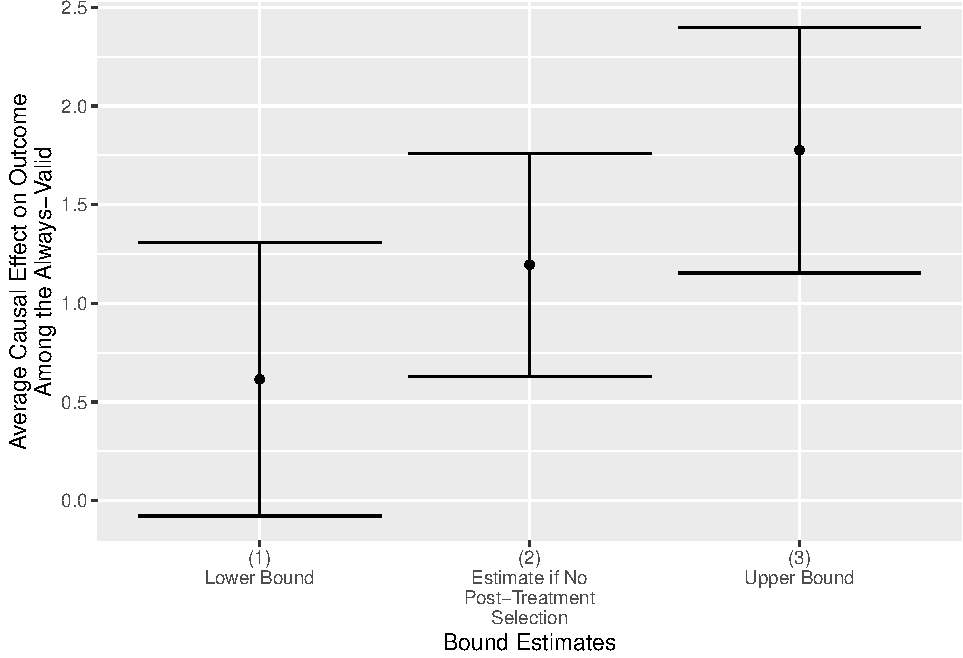
\includegraphics{05_se_files/figure-latex/unnamed-chunk-6-1.pdf}

\hypertarget{glossary-of-estimands-that-result}{%
\section{Glossary of estimands that result}\label{glossary-of-estimands-that-result}}

\begin{longtable}[]{@{}
  >{\centering\arraybackslash}p{(\columnwidth - 4\tabcolsep) * \real{0.3333}}
  >{\centering\arraybackslash}p{(\columnwidth - 4\tabcolsep) * \real{0.3333}}
  >{\centering\arraybackslash}p{(\columnwidth - 4\tabcolsep) * \real{0.3333}}@{}}
\toprule\noalign{}
\begin{minipage}[b]{\linewidth}\centering
Value of \texttt{estimand}
\end{minipage} & \begin{minipage}[b]{\linewidth}\centering
Definition
\end{minipage} & \begin{minipage}[b]{\linewidth}\centering
English
\end{minipage} \\
\midrule\noalign{}
\endhead
\bottomrule\noalign{}
\endlastfoot
\texttt{effect\_y\_naive} & \(\hat{E}_{\text{Naive}}(Y^1-Y^0\mid S = \text{Always})\) & Average effect of treatment on outcome in always-valid stratum, estimated by assumption that potential outcomes are conditionally independent of \(M\) \\
\texttt{effect\_y\_lower} & \(\hat{E}_{\text{Lower}}(Y^1-Y^0\mid S = \text{Always})\) & Lower bound average effect of treatment on outcome in always-valid stratum \\
\texttt{effect\_y\_upper} & \(\hat{E}_{\text{Lower}}(Y^1-Y^0\mid S = \text{Always})\) & Upper bound average effect of treatment on outcome in always-valid stratum \\
\texttt{yhat\_1\_naive} & \(\hat{E}_{\text{Naive}}(Y^1\mid S = \text{Always})\) & Average outcome under treatment in the always-valid stratum, estimated by assumption potential outcomes are conditionally independent of \(M\) \\
\texttt{yhat\_0\_naive} & \(\hat{E}_{\text{Naive}}(Y^0\mid S = \text{Always})\) & Analogous to above, for outcome under control \\
\texttt{yhat\_1\_lower} & \(\hat{E}_{\text{Lower}}(Y^1\mid S = \text{Always})\) & Lower bound average outcome under treatment in the always-valid stratum \\
\texttt{yhat\_0\_lower} & \(\hat{E}_{\text{Lower}}(Y^0\mid S = \text{Always})\) & Analogous to above, for outcome under control \\
\texttt{yhat\_1\_upper} & \(\hat{E}_{\text{Upper}}(Y^1\mid S = \text{Always})\) & Upper bound average outcome under treatment in the always-valid stratum \\
\texttt{yhat\_0\_upper} & \(\hat{E}_{\text{Upper}}(Y^0\mid S = \text{Always})\) & Analogous to above, for outcome under control \\
\texttt{effect\_m} & \(\hat{E}(M^1-M^0)\) & Average effect of treatment on mediator \\
\texttt{mhat1} & \(\hat{E}(M^1)\) & Average mediator under treatment \\
\texttt{mhat1\_trunc} & & The above, truncated to comply with the user-defined positivity assumption \\
\texttt{mhat0} & \(\hat{E}(M^0)\) & Average mediator under control \\
\texttt{mhat0\_trunc} & & The above, truncated to comply with the user-defined positivity assumption \\
\end{longtable}

  \bibliography{book.bib,packages.bib}

\end{document}
